\documentclass[a4paper,10pt]{article}\usepackage[]{graphicx}\usepackage[]{xcolor}
% maxwidth is the original width if it is less than linewidth
% otherwise use linewidth (to make sure the graphics do not exceed the margin)
\makeatletter
\def\maxwidth{ %
  \ifdim\Gin@nat@width>\linewidth
    \linewidth
  \else
    \Gin@nat@width
  \fi
}
\makeatother

\definecolor{fgcolor}{rgb}{0.345, 0.345, 0.345}
\newcommand{\hlnum}[1]{\textcolor[rgb]{0.686,0.059,0.569}{#1}}%
\newcommand{\hlsng}[1]{\textcolor[rgb]{0.192,0.494,0.8}{#1}}%
\newcommand{\hlcom}[1]{\textcolor[rgb]{0.678,0.584,0.686}{\textit{#1}}}%
\newcommand{\hlopt}[1]{\textcolor[rgb]{0,0,0}{#1}}%
\newcommand{\hldef}[1]{\textcolor[rgb]{0.345,0.345,0.345}{#1}}%
\newcommand{\hlkwa}[1]{\textcolor[rgb]{0.161,0.373,0.58}{\textbf{#1}}}%
\newcommand{\hlkwb}[1]{\textcolor[rgb]{0.69,0.353,0.396}{#1}}%
\newcommand{\hlkwc}[1]{\textcolor[rgb]{0.333,0.667,0.333}{#1}}%
\newcommand{\hlkwd}[1]{\textcolor[rgb]{0.737,0.353,0.396}{\textbf{#1}}}%
\let\hlipl\hlkwb

\usepackage{framed}
\makeatletter
\newenvironment{kframe}{%
 \def\at@end@of@kframe{}%
 \ifinner\ifhmode%
  \def\at@end@of@kframe{\end{minipage}}%
  \begin{minipage}{\columnwidth}%
 \fi\fi%
 \def\FrameCommand##1{\hskip\@totalleftmargin \hskip-\fboxsep
 \colorbox{shadecolor}{##1}\hskip-\fboxsep
     % There is no \\@totalrightmargin, so:
     \hskip-\linewidth \hskip-\@totalleftmargin \hskip\columnwidth}%
 \MakeFramed {\advance\hsize-\width
   \@totalleftmargin\z@ \linewidth\hsize
   \@setminipage}}%
 {\par\unskip\endMakeFramed%
 \at@end@of@kframe}
\makeatother

\definecolor{shadecolor}{rgb}{.97, .97, .97}
\definecolor{messagecolor}{rgb}{0, 0, 0}
\definecolor{warningcolor}{rgb}{1, 0, 1}
\definecolor{errorcolor}{rgb}{1, 0, 0}
\newenvironment{knitrout}{}{} % an empty environment to be redefined in TeX

\usepackage{alltt}
\usepackage[utf8]{inputenc}
\usepackage[margin=2.5cm]{geometry}
\usepackage{float}

\title{Estadística en les Ciències de la Salut \\ Assignment 1; Group 03}
\author{1711342 Roger Guitart Casals; 1707055 Sergi Resina Xirgo \\ 1705323 Lucca Bergonzini Flores; 1702697 Àlex Vega Tomàs}
\date{28/10/2026}
\IfFileExists{upquote.sty}{\usepackage{upquote}}{}
\begin{document}
%\SweaveOpts{concordance=TRUE}
\maketitle

\section{Introduction}

In this study we will investigate how to use R packages such as mice and miclust to apply statistical tools for missing data. Our goal is to generate clusters to analyze and visualize our dataset. This dataset is a subset of the variables studied in the original paper by Basagaña et al.\cite{paper}


\section{Analysis}
\subsection{Description of missingness}




\begin{knitrout}
\definecolor{shadecolor}{rgb}{0.969, 0.969, 0.969}\color{fgcolor}\begin{kframe}
\begin{alltt}
\hldef{n_participants} \hlkwb{<-} \hlkwd{nrow}\hldef{(copd)}
\hldef{n_variables} \hlkwb{<-} \hlkwd{ncol}\hldef{(copd)}
\hldef{missing_per_variable} \hlkwb{<-} \hlkwd{colMeans}\hldef{(}\hlkwd{is.na}\hldef{(copd))} \hlopt{*} \hlnum{100}

\hldef{min_missing} \hlkwb{<-} \hlkwd{sprintf}\hldef{(}\hlsng{"%.1f"}\hldef{,} \hlkwd{min}\hldef{(missing_per_variable))}
\hldef{max_missing} \hlkwb{<-} \hlkwd{sprintf}\hldef{(}\hlsng{"%.1f"}\hldef{,} \hlkwd{max}\hldef{(missing_per_variable))}

\hldef{pct_variables_lt5} \hlkwb{<-} \hlkwd{sprintf}\hldef{(}\hlsng{"%.1f"}\hldef{,} \hlkwd{mean}\hldef{(missing_per_variable} \hlopt{<} \hlnum{5}\hldef{)} \hlopt{*} \hlnum{100}\hldef{)} \hlcom{# mean}
\hlcom{# computes the proportion of TRUE values}
\hlcom{# equivalent: AA <- sprintf("%.1f", sum((missing_per_variable < 5))/n_variables * 100)}
\hlcom{# true=1, false=0}

\hldef{pct_complete_cases} \hlkwb{<-} \hlkwd{sprintf}\hldef{(}\hlsng{"%.1f"}\hldef{,} \hlkwd{mean}\hldef{(}\hlkwd{complete.cases}\hldef{(copd))} \hlopt{*} \hlnum{100}\hldef{)}
\hldef{pct_missing_total} \hlkwb{<-} \hlkwd{sprintf}\hldef{(}\hlsng{"%.1f"}\hldef{,} \hlkwd{mean}\hldef{(}\hlkwd{is.na}\hldef{(}\hlkwd{as.matrix}\hldef{(copd)))} \hlopt{*} \hlnum{100}\hldef{)}

\hldef{total_cells} \hlkwb{<-} \hlkwd{prettyNum}\hldef{(n_participants} \hlopt{*} \hldef{n_variables,} \hlkwc{big.mark}\hldef{=}\hlsng{","}\hldef{)} \hlcom{# n_participants}
                                                    \hlcom{# * n_variables = total_cells}
\end{alltt}
\end{kframe}
\end{knitrout}

The subset used here included 342 participants and 45 variables. The range of missing data in the different variables went from 0.0\% to 31.6\%, with 68.9\% of the variables having less than 5\% of the data missing. Only 33.3\% of the participants had complete data on all 45 variables. Overall, 5.4\% of the information was missing; that is, 5.4\% of the total of
15,390 cells (45 x 342 = 15,390) had missing data.

\subsection{Multiple imputation}
Apply multiple imputation to copd data using 100 imputations. Explain in a reasoned
manner how you decided to set the values of the arguments method and predictorMatrix
when using the mice() function. Show your code



\begin{knitrout}
\definecolor{shadecolor}{rgb}{0.969, 0.969, 0.969}\color{fgcolor}\begin{kframe}
\begin{alltt}
\hldef{ini} \hlkwb{<-} \hlkwd{mice}\hldef{(copd,} \hlkwc{maxit} \hldef{=} \hlnum{0}\hldef{)}

\hldef{meth} \hlkwb{<-} \hldef{ini}\hlopt{$}\hldef{method}
\hldef{pred} \hlkwb{<-} \hldef{ini}\hlopt{$}\hldef{predictorMatrix}

\hldef{meth[}\hlsng{"id"}\hldef{]} \hlkwb{<-} \hlsng{""} \hlcom{# do not impute "id"}
\hldef{pred[}\hlsng{"id"}\hldef{, ]} \hlkwb{<-} \hlnum{0} \hlcom{# we don't want "id" to be imputed}
\hldef{pred[,} \hlsng{"id"}\hldef{]} \hlkwb{<-} \hlnum{0} \hlcom{# we don't want "id" to be predictor}

\hlcom{# Perform the 100 imputations:}
\hldef{imp} \hlkwb{<-} \hlkwd{mice}\hldef{(copd,} \hlkwc{method} \hldef{= meth,} \hlkwc{predictorMatrix} \hldef{= pred,} \hlkwc{m} \hldef{=} \hlnum{100}\hldef{,}
            \hlkwc{printFlag} \hldef{=} \hlnum{FALSE}\hldef{,} \hlkwc{seed} \hldef{=} \hlnum{123}\hldef{)}
\end{alltt}
\end{kframe}
\end{knitrout}

We kept the same methodology and the predictor matrix, with the exception of id as it isn't relevant for this process.
The variable 'm' encodes the number of imputations, 'printFlag' is used to show the current imputation although it's not important for the results,
and the 'seed' is set up for replicability. 


\subsection{Integration of multiple imputation in cluster analysis}

Reproduce the original analysis in the paper using the miclust package to integrate multiple
imputation in the cluster analysis. Apply the proposed framework using the same setting
as in the original analysis.

To do that, follow these steps:


1. Read the help of the getdata() function in the miclust package. Then, accordingly,
create a list of data.frames and pass it to the getdata() function. Give a detailed
explanation of the data processing you did to get that list. Show your code.

\begin{knitrout}
\definecolor{shadecolor}{rgb}{0.969, 0.969, 0.969}\color{fgcolor}\begin{kframe}
\begin{alltt}
\hldef{resultat_mice} \hlkwb{<-} \hlkwd{complete}\hldef{(imp,} \hlkwc{action} \hldef{=} \hlsng{"all"}\hldef{,} \hlkwc{include} \hldef{=} \hlnum{TRUE}\hldef{)}
\hlcom{# action = "all" already puts the original data as the first element}

\hldef{categoriques} \hlkwb{<-} \hlkwd{c}\hldef{(}
  \hlsng{"sin11_v1"}\hldef{,} \hlsng{"iam_chv1"}\hldef{,} \hlsng{"sin15_v1"}\hldef{,} \hlsng{"sin7_v1"}\hldef{,} \hlsng{"sin8_v1"}\hldef{,}
  \hlsng{"cccs1_v0"}\hldef{,} \hlsng{"vtit_catv1"}\hldef{,} \hlsng{"urg_ambv0"}\hldef{,} \hlsng{"sin5_v1"}\hldef{,}
  \hlsng{"sin6_v1"}\hldef{,} \hlsng{"graudisn_v1"}
\hldef{)}

\hldef{resultat_mice} \hlkwb{<-} \hlkwd{lapply}\hldef{(resultat_mice,} \hlkwa{function}\hldef{(}\hlkwc{d}\hldef{) \{}
  \hldef{d}\hlopt{$}\hldef{id} \hlkwb{<-} \hlkwa{NULL}
  \hldef{d[categoriques]} \hlkwb{<-} \hlkwd{lapply}\hldef{(d[categoriques],} \hlkwa{function}\hldef{(}\hlkwc{x}\hldef{)}
    \hlkwd{as.numeric}\hldef{(}\hlkwd{as.character}\hldef{(x)))}
  \hldef{d}
\hldef{\})}

\hldef{miclustdata} \hlkwb{<-} \hlkwd{getdata}\hldef{(resultat_mice)} \hlcom{# adapts the data to the miclust format}
\end{alltt}
\end{kframe}
\end{knitrout}

As 'getdata()' necessitates a list of dataframes, where the first
element has the initial data and the imputations are stored in the subsequent elements,
we call the 'complete' function that returns the needed information when using
"action=all" and "include=TRUE". Furthermore, we must adapt the categorical
variables to numerical values. Thus we define a function that transforms the values stored
in text into numbers and using the 'lapply()' function, we reach our goal: the list of dataframes that 'getdata()' needs.


2. Use the miclust() function to perform the integration of missing data in cluster
analysis using the same settings as in the original analysis. Show your code and
explain how and why you set all arguments in the miclust() function.

\begin{knitrout}
\definecolor{shadecolor}{rgb}{0.969, 0.969, 0.969}\color{fgcolor}\begin{kframe}
\begin{alltt}
\hlcom{# Second part:}
\hldef{copd_miclustdata} \hlkwb{<-} \hlkwd{miclust}\hldef{(}\hlkwc{data} \hldef{= miclustdata,}\hlkwc{search} \hldef{=} \hlsng{"backward"}\hldef{,}
                            \hlkwc{ks} \hldef{=} \hlnum{2}\hlopt{:}\hlnum{3}\hldef{,}
                            \hlkwc{distance} \hldef{=} \hlsng{"manhattan"}\hldef{,}
                            \hlkwc{centpos} \hldef{=} \hlsng{"means"}\hldef{,}
                            \hlkwc{initcl} \hldef{=} \hlsng{"hc"}\hldef{,}
                            \hlkwc{verbose} \hldef{=} \hlnum{TRUE}\hldef{,}
                            \hlkwc{seed} \hldef{=} \hlnum{123}\hldef{)}
\end{alltt}
\begin{verbatim}
## . . . . imp   5 . . . . imp  10 . . . . imp  15 . . . . imp  20 
## . . . . imp  25 . . . . imp  30 . . . . imp  35 . . . . imp  40 
## . . . . imp  45 . . . . imp  50 . . . . imp  55 . . . . imp  60 
## . . . . imp  65 . . . . imp  70 . . . . imp  75 . . . . imp  80 
## . . . . imp  85 . . . . imp  90 . . . . imp  95 . . . . imp 100 
## 
##  Analysis done.
\end{verbatim}
\end{kframe}
\end{knitrout}


The chosen elements have been: 'backward', because we were instructed to
during class; 'ks = 2:3', as the paper itself led us to believe that a high
number of clusters would lead to inaccurate  results; 'manhattan', the default
option; 'means', as we are using the k-means algorithm; 'hc', we decided on 
a hierarchical initialization over a random one for better results;
'verbose = TRUE', to show the progress of this long process; 'seed=123' for replicability.


\section{Results}
Using plot() and summary() methods in the miclust package, provide plots\textsubscript{1} and tables
for the results similar to those shown in the original paper. Also, show a barplot for the
percentage of times each variable is selected among the imputed data sets, in decreasing
order\textsubscript{2}. Explain how you set all arguments in all functions and methods you use. Show
your code.


\begin{knitrout}
\definecolor{shadecolor}{rgb}{0.969, 0.969, 0.969}\color{fgcolor}\begin{kframe}
\begin{alltt}
\hlkwd{plot}\hldef{(copd_miclustdata,} \hlkwc{metric}\hldef{=}\hlsng{"nclfreq"}\hldef{,} \hlkwc{col.nclfreq} \hldef{=} \hlsng{"blue"}\hldef{)}
\end{alltt}
\end{kframe}\begin{figure}[H]
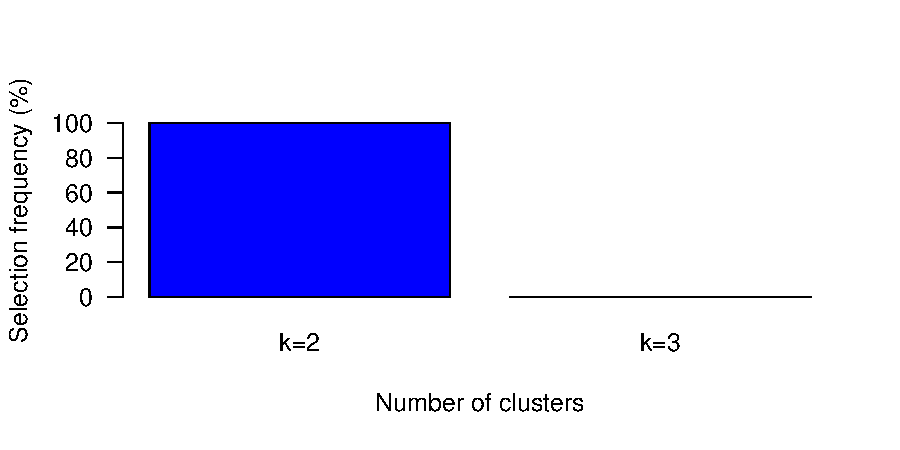
\includegraphics[width=\maxwidth]{figure/plot1-1} \caption[Number of clusters frequency]{Number of clusters frequency}\label{fig:plot1}
\end{figure}

\end{knitrout}

\begin{knitrout}
\definecolor{shadecolor}{rgb}{0.969, 0.969, 0.969}\color{fgcolor}\begin{kframe}
\begin{alltt}
\hlkwd{plot}\hldef{(copd_miclustdata,} \hlkwc{metric}\hldef{=}\hlsng{"critcf"}\hldef{,} \hlkwc{col.critcf} \hldef{=} \hlsng{"orange"}\hldef{)}
\end{alltt}
\end{kframe}\begin{figure}[H]
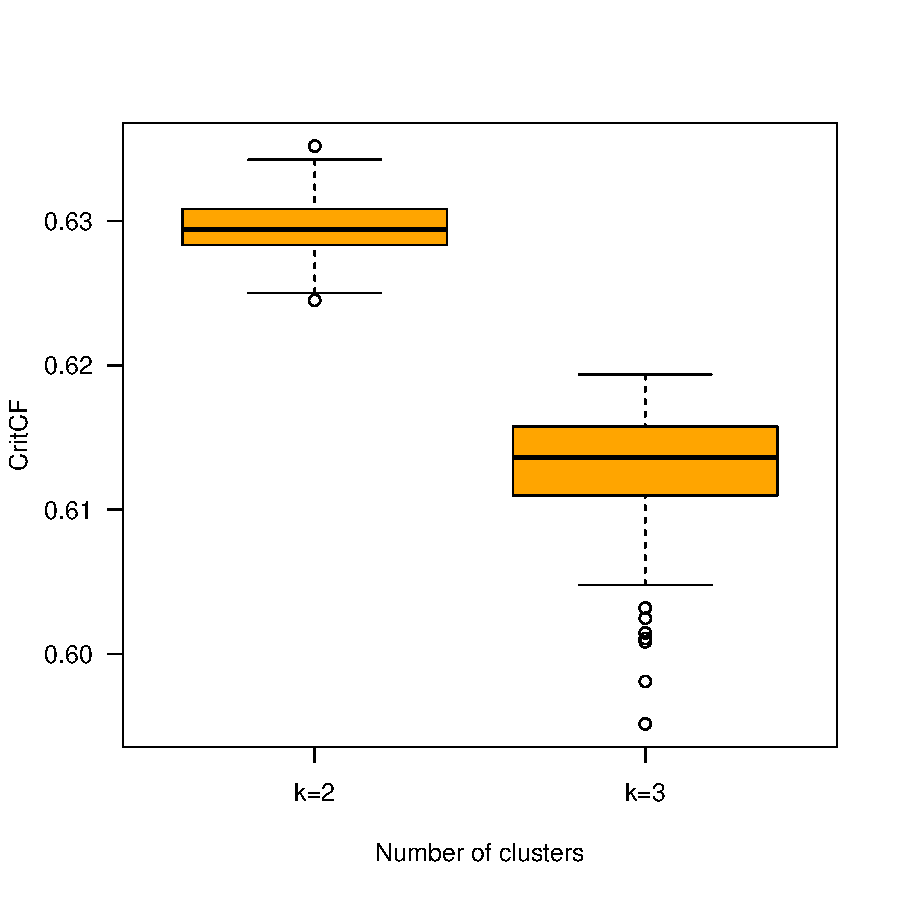
\includegraphics[width=\maxwidth]{figure/plot2-1} \caption[CritCF value versus number of clusters]{CritCF value versus number of clusters}\label{fig:plot2}
\end{figure}

\end{knitrout}

\begin{knitrout}
\definecolor{shadecolor}{rgb}{0.969, 0.969, 0.969}\color{fgcolor}\begin{kframe}
\begin{alltt}
\hlkwd{plot}\hldef{(copd_miclustdata,} \hlkwc{metric}\hldef{=}\hlsng{"nvarfreq"}\hldef{,} \hlkwc{col.nvarfreq} \hldef{=} \hlsng{"forestgreen"}\hldef{)}
\end{alltt}
\end{kframe}\begin{figure}[H]
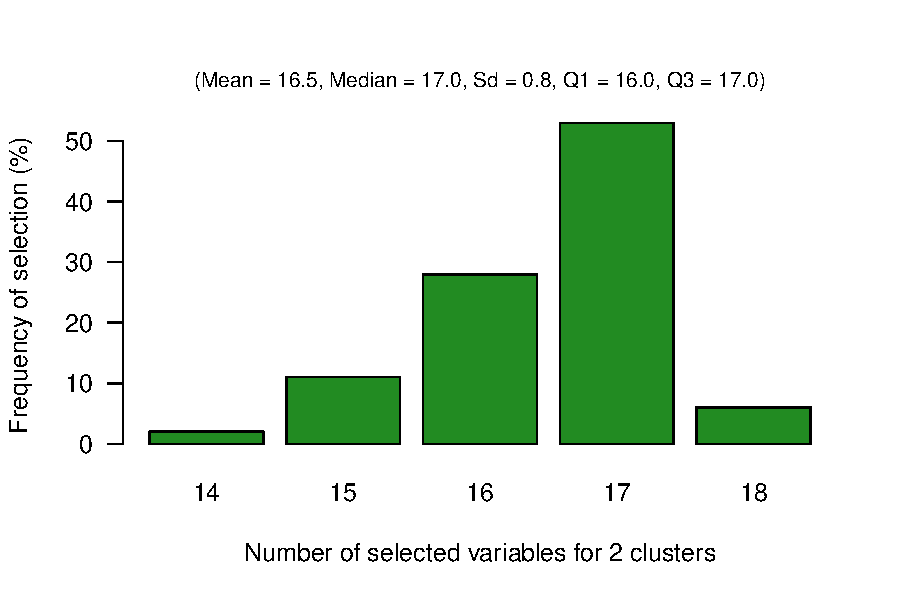
\includegraphics[width=\maxwidth]{figure/plot3-1} \caption[Frequency of the number of times each variable being selected furing multiple imputation]{Frequency of the number of times each variable being selected furing multiple imputation}\label{fig:plot3}
\end{figure}

\end{knitrout}

\begin{knitrout}
\definecolor{shadecolor}{rgb}{0.969, 0.969, 0.969}\color{fgcolor}\begin{kframe}
\begin{alltt}
\hlkwd{plot}\hldef{(copd_miclustdata,} \hlkwc{metric}\hldef{=}\hlsng{"varsel"}\hldef{,} \hlkwc{col.varsel} \hldef{=} \hlsng{"gray"}\hldef{)}
\end{alltt}
\end{kframe}\begin{figure}[H]
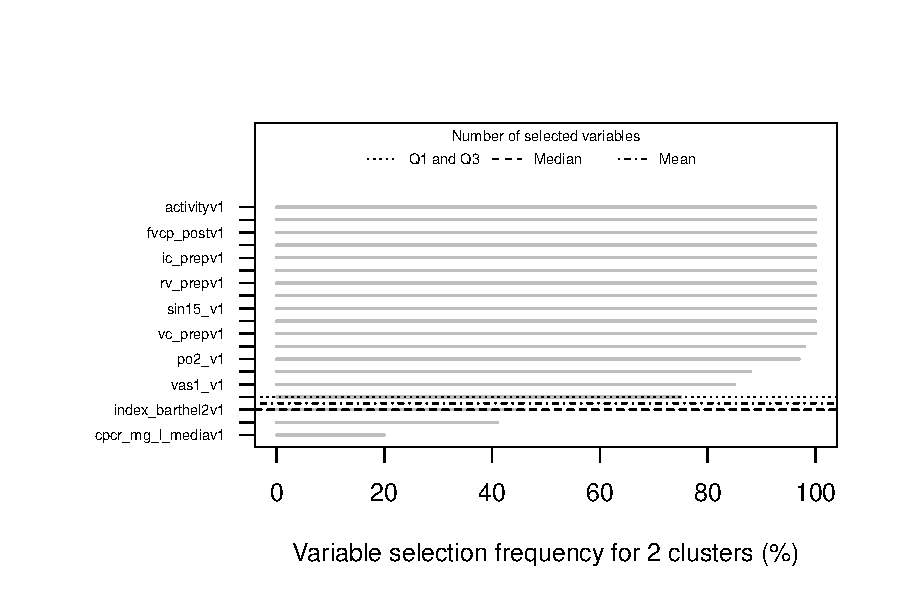
\includegraphics[width=\maxwidth]{figure/plot4-1} \caption[Frequency of each variable being selected during multiple imputation]{Frequency of each variable being selected during multiple imputation}\label{fig:plot4}
\end{figure}

\end{knitrout}

We only needed to define the colors to show the plots.


\begin{kframe}
\begin{alltt}
\hldef{res2} \hlkwb{<-} \hlkwd{summary}\hldef{(copd_miclustdata,} \hlkwc{k} \hldef{=} \hlnum{2}\hldef{,} \hlkwc{quantilevars} \hldef{=} \hlnum{0.5}\hldef{)}
\hldef{res3} \hlkwb{<-} \hlkwd{summary}\hldef{(copd_miclustdata,} \hlkwc{k} \hldef{=} \hlnum{3}\hldef{,} \hlkwc{quantilevars} \hldef{=} \hlnum{0.5}\hldef{)}

\hldef{resum_prob} \hlkwb{<-} \hlkwd{rbind}\hldef{(res2}\hlopt{$}\hldef{allocationprobabilities, res3}\hlopt{$}\hldef{allocationprobabilities)}

\hlkwd{rownames}\hldef{(resum_prob)} \hlkwb{<-} \hlkwd{c}\hldef{(}\hlsng{"k = 2, Cluster 1"}\hldef{,}
                          \hlsng{"k = 2, Cluster 2"}\hldef{,}
                          \hlsng{"k = 3, Cluster 1"}\hldef{,}
                          \hlsng{"k = 3, Cluster 2"}\hldef{,}
                          \hlsng{"k = 3, Cluster 3"}\hldef{)}

\hldef{modtable} \hlkwb{<-} \hlkwd{xtable}\hldef{(resum_prob,}
                   \hlkwc{digits} \hldef{=} \hlkwd{c}\hldef{(}\hlnum{0}\hldef{,} \hlnum{3}\hldef{,} \hlnum{3}\hldef{,} \hlnum{3}\hldef{,} \hlnum{3}\hldef{,} \hlnum{3}\hldef{),}
                   \hlkwc{caption} \hldef{=} \hlsng{"Distribution of the Frequencies of Assignment
                   (Proportions) for Each Cluster (for k = 2 and k = 3)"}\hldef{,}
                   \hlkwc{label} \hldef{=} \hlsng{"tab:frequency"}\hldef{)}
\hlcom{# cosmetics for table head (LaTeX slash (\textbackslash{}) must be doubled inside a R chunk):}
\hlkwd{colnames}\hldef{(modtable)} \hlkwb{<-} \hlkwd{c}\hldef{(}\hlsng{"\textbackslash{}\textbackslash{}multicolumn\{1\}\{c\}\{\textbackslash{}\textbackslash{}bf Minimum\}"}\hldef{,}
                        \hlsng{"\textbackslash{}\textbackslash{}multicolumn\{1\}\{c\}\{\textbackslash{}\textbackslash{}bf First Quartile\}"}\hldef{,}
                        \hlsng{"\textbackslash{}\textbackslash{}multicolumn\{1\}\{c\}\{\textbackslash{}\textbackslash{}bf Median\}"}\hldef{,}
                        \hlsng{"\textbackslash{}\textbackslash{}multicolumn\{1\}\{c\}\{\textbackslash{}\textbackslash{}bf Third Quartile\}"}\hldef{,}
                        \hlsng{"\textbackslash{}\textbackslash{}multicolumn\{1\}\{c\}\{\textbackslash{}\textbackslash{}bf Maximum\}"}\hldef{)}

\hlcom{# format and print the table:}
\hlkwd{print}\hldef{(modtable,}
      \hlkwc{table.placement} \hldef{=} \hlsng{"ht"}\hldef{,}
      \hlkwc{size} \hldef{=} \hlsng{"footnotesize"}\hldef{,}
      \hlkwc{include.rownames} \hldef{=} \hlnum{TRUE}\hldef{,}
      \hlkwc{include.colnames} \hldef{=} \hlnum{TRUE}\hldef{,}
      \hlkwc{floating} \hldef{=} \hlnum{TRUE}\hldef{,}                 \hlcom{# whether \textbackslash{}begin\{table\}}
      \hlcom{# should be created (TRUE) or not (FALSE)}
      \hlcom{# important to treat content}
      \hlcom{# of columns as latex function}
      \hlkwc{sanitize.text.function} \hldef{= force)}
\end{alltt}
\end{kframe}% latex table generated in R 4.6.1 by xtable 1.8-8 package
% Wed Oct 28 22:06:23 2026
\begin{table}[ht]
\centering
\begingroup\footnotesize
\begin{tabular}{rrrrrr}
  \hline
 & \multicolumn{1}{c}{\bf Minimum} & \multicolumn{1}{c}{\bf First Quartile} & \multicolumn{1}{c}{\bf Median} & \multicolumn{1}{c}{\bf Third Quartile} & \multicolumn{1}{c}{\bf Maximum} \\ 
  \hline
k = 2, Cluster 1 & 0.520 & 1.000 & 1.000 & 1.000 & 1.000 \\ 
  k = 2, Cluster 2 & 0.540 & 1.000 & 1.000 & 1.000 & 1.000 \\ 
  k = 3, Cluster 1 & 0.600 & 1.000 & 1.000 & 1.000 & 1.000 \\ 
  k = 3, Cluster 2 & 0.500 & 1.000 & 1.000 & 1.000 & 1.000 \\ 
  k = 3, Cluster 3 & 0.540 & 1.000 & 1.000 & 1.000 & 1.000 \\ 
   \hline
\end{tabular}
\endgroup
\caption{Distribution of the Frequencies of Assignment
                   (Proportions) for Each Cluster (for k = 2 and k = 3)} 
\label{tab:frequency}
\end{table}


Answer: To create the first table we use the 'summary()' function for the
different k-values, and using a template provided by the professor, we show the
desired results.

\begin{kframe}
\begin{alltt}
\hldef{descr} \hlkwb{<-} \hlkwd{as.data.frame}\hldef{(res2}\hlopt{$}\hldef{summarybycluster)}

\hldef{taula3} \hlkwb{<-} \hlkwd{data.frame}\hldef{(}\hlkwc{Variable} \hldef{=} \hlkwd{gsub}\hldef{(}\hlsng{"_"}\hldef{,} \hlsng{"\textbackslash{}\textbackslash{}\textbackslash{}\textbackslash{}_"}\hldef{,} \hlkwd{rownames}\hldef{(descr)),}
                     \hlkwc{Missing} \hldef{=} \hlkwd{as.numeric}\hldef{(descr[[}\hlsng{"%miss."}\hldef{]]),}
                     \hlkwc{Cluster1} \hldef{=} \hlkwd{as.numeric}\hldef{(descr[[}\hlsng{"mean (cl.1)"}\hldef{]]),}
                     \hlkwc{Cluster2} \hldef{=} \hlkwd{as.numeric}\hldef{(descr[[}\hlsng{"mean (cl.2)"}\hldef{]]),}
                     \hlkwc{check.names} \hldef{=} \hlnum{FALSE}
\hldef{)}

\hldef{n} \hlkwb{<-} \hldef{res2}\hlopt{$}\hldef{clusterssize[,} \hlsng{"50%"}\hldef{]} \hlcom{# Value of the median cluster size}

\hldef{modtable} \hlkwb{<-} \hlkwd{xtable}\hldef{(taula3,}
                   \hlkwc{digits} \hldef{=} \hlkwd{c}\hldef{(}\hlnum{0}\hldef{,} \hlnum{0}\hldef{,} \hlnum{2}\hldef{,} \hlnum{2}\hldef{,} \hlnum{2}\hldef{),}
                   \hlkwc{caption} \hldef{=} \hlsng{"Description of the Variables (Mean Values) by Cluster"}\hldef{,}
                   \hlkwc{label} \hldef{=} \hlsng{"tab:descr"}\hldef{)}
\hlcom{# cosmetics for table head (LaTeX slash (\textbackslash{}) must be doubled inside a R chunk):}
\hlkwd{colnames}\hldef{(modtable)} \hlkwb{<-} \hlkwd{c}\hldef{(}\hlsng{"\textbackslash{}\textbackslash{}multicolumn\{1\}\{c\}\{\textbackslash{}\textbackslash{}bf Variable\}"}\hldef{,}
                        \hlsng{"\textbackslash{}\textbackslash{}multicolumn\{1\}\{c\}\{\textbackslash{}\textbackslash{}bf \textbackslash{}\textbackslash{}% of Subjects With Missing Values\}"}\hldef{,}
                        \hlkwd{paste0}\hldef{(}\hlsng{"\textbackslash{}\textbackslash{}multicolumn\{1\}\{c\}\{\textbackslash{}\textbackslash{}bf Cluster 1 (n = "}\hldef{, n[}\hlnum{1}\hldef{],} \hlsng{")\}"}\hldef{),}
                        \hlcom{# paste0 to concatenate strings}
                        \hlkwd{paste0}\hldef{(}\hlsng{"\textbackslash{}\textbackslash{}multicolumn\{1\}\{c\}\{\textbackslash{}\textbackslash{}bf Cluster 2 (n = "}\hldef{, n[}\hlnum{2}\hldef{],} \hlsng{")\}"}\hldef{))}

\hlcom{# format and print the table:}
\hlkwd{print}\hldef{(modtable,}
      \hlkwc{table.placement} \hldef{=} \hlsng{"ht"}\hldef{,}
      \hlkwc{size} \hldef{=} \hlsng{"footnotesize"}\hldef{,}
      \hlkwc{include.rownames} \hldef{=} \hlnum{FALSE}\hldef{,}
      \hlkwc{include.colnames} \hldef{=} \hlnum{TRUE}\hldef{,}
      \hlcom{# whether \textbackslash{}begin\{table\} should be created (TRUE) or not (FALSE)}
      \hlkwc{floating} \hldef{=} \hlnum{TRUE}\hldef{,}
      \hlcom{# important to treat content of columns as latex function}
      \hlkwc{sanitize.text.function} \hldef{= force)}
\end{alltt}
\end{kframe}% latex table generated in R 4.6.1 by xtable 1.8-8 package
% Wed Oct 28 22:06:24 2026
\begin{table}[ht]
\centering
\begingroup\footnotesize
\begin{tabular}{lrrr}
  \hline
\multicolumn{1}{c}{\bf Variable} & \multicolumn{1}{c}{\bf \% of Subjects With Missing Values} & \multicolumn{1}{c}{\bf Cluster 1 (n = 186)} & \multicolumn{1}{c}{\bf Cluster 2 (n = 156)} \\ 
  \hline
activityv1 & 1.17 & 35.80 & 60.79 \\ 
  fevp\_postv1 & 0.00 & 62.74 & 39.12 \\ 
  fvcp\_postv1 & 0.00 & 79.93 & 63.65 \\ 
  iam\_chv1 & 0.88 & 0.12 & 0.08 \\ 
  ic\_prepv1 & 5.56 & 72.84 & 52.43 \\ 
  quo\_calcpostv1 & 0.00 & 58.83 & 45.89 \\ 
  rv\_prepv1 & 7.89 & 138.51 & 184.77 \\ 
  rv\_tlcv1 & 7.89 & 50.89 & 63.19 \\ 
  sin15\_v1 & 1.17 & 0.09 & 0.09 \\ 
  vas2\_v1 & 1.17 & 4.18 & 6.49 \\ 
  vc\_prepv1 & 5.56 & 77.48 & 60.45 \\ 
  impactsv1 & 1.17 & 18.61 & 35.81 \\ 
  po2\_v1 & 3.22 & 77.39 & 69.67 \\ 
  graudisn\_v1 & 1.17 & 1.91 & 3.27 \\ 
  vas1\_v1 & 1.17 & 2.00 & 3.98 \\ 
  cccs1\_v0 & 1.46 & 0.15 & 0.18 \\ 
  index\_barthel2v1 & 2.63 & 100.00 & 98.15 \\ 
   \hline
\end{tabular}
\endgroup
\caption{Description of the Variables (Mean Values) by Cluster} 
\label{tab:descr}
\end{table}


We haven't included the 'F values' in the second table, nor used
the unprocessed data for the average-value analysis, but we have decided to
show other results from the 'summary()' function, which we considered relevant
to the imputed data. To do this, an auxiliary dataframe of the 'summary' was
needed. Furthermore, we obtained the mean value of the clusters just like the 
original paper did.

\section{Report}

The final analysis divided the dataset into \textbf{2 clusters}. We can see in
Figure~\ref{fig:plot1} that k=2 (having 2 clusters) is chosen every time, thus we can
conclude without uncertainty that we can divide the dataset into two clusters.
Table~\ref{tab:descr} details the size of each of these clusters: n=186 for the first
cluster and n=156 for the second one.

The relabeling of the clusters over multiple imputations (the same cluster being
labelled differently in different imputations) is handled internally by the
\textbf{miclust} package, as detailed in its documentation. \cite{source_code}

Figure~\ref{fig:plot3} shows how many variables were selected across the
imputations: an average of 16.5, with a median of 17, standard deviation of
0.8 and an interquartile range of 16-17. Thus, the final subset contains 17
variables and the uncertainty over this choice is low.
Figure~\ref{fig:plot4} shows us the selection frequency for each variable: the
most selected include activityv1, fvcp\_postv1, ic\_prepv1, rv\_prepv1, sin15\_v1,
vc\_prepv1, po2\_v1, vas1\_v1, index\_barthel2v1 and cpcr\_mg\_l\_mediav1. Table~\ref{tab:descr}
lists the variables used in the descriptive cluster.

In Table~\ref{tab:frequency}, we can see that, for each cluster when k = 2 and k = 3, at least
three-quarters of its instances are assigned to the same cluster across all imputations. 
Therefore, assuming that the missing data follow the proposed distributions, at least 75\% 
of all instances don't have uncertainty.




\section{Use of artificial intelligence}

Artificial Intelligence, more accurately Large Language Models (LLMs), have been
used to revise and enhance the code displayed in this paper. Here is the exact
prompt and answer of the one time they were used:

\textbf{Prompt:} 

\begin{verbatim}
Tinc aquest codi en R:
resultat_mice<-complete(imp, action="all", include=TRUE)
categorics_amb_ordre <- c("sin11_v1", "iam_chv1", "sin15_v1", "sin7_v1",
"sin8_v1","cccs1_v0", "vtit_catv1", "urg_ambv0", "sin5_v1", "sin6_v1")
categorics_sense_ordre <- c("graudisn_v1")
for (i in 1:(M+1))
{
  for (j in categorics_amb_ordre)
  {
    resultat_mice[[i]][[j]] <- as.numeric(levels(resultat_mice[[i]][[j]]))
    [resultat_mice[[i]][[j]]]
  }
  for (j in categorics_sense_ordre)
  {
    resultat_mice[[i]][[j]] <- as.numeric(levels(resultat_mice[[i]][[j]]))
    [resultat_mice[[i]][[j]]]
  }
}
miclustdata<-getdata(resultat_mice)


Saps si es pot optimitzar i simplificar? També voldria eliminar la columna
id de cada conjunt de dades imputat abans de crear miclustdata.
\end{verbatim}



\textbf{Answer:}

\begin{verbatim}
Sí. En el teu codi original hi ha dues simplificacions clares:

1. categorics_amb_ordre i categorics_sense_ordre reben exactament el mateix tractament,
   per tant es poden unir en un únic vector.
2. Es poden evitar els for utilitzant lapply(), cosa que fa el codi
   més compacte i independent de M.
3. Pots eliminar la columna id dins del mateix procés.

Una possible versió simplificada seria:


resultat_mice <- complete(imp, action = "all", include = TRUE)


categoriques <- c(
  "sin11_v1", "iam_chv1", "sin15_v1", "sin7_v1", "sin8_v1",
  "cccs1_v0", "vtit_catv1", "urg_ambv0", "sin5_v1",
  "sin6_v1", "graudisn_v1"
)

resultat_mice <- lapply(resultat_mice, function(d) {

  # Eliminar la variable identificadora
  d$id <- NULL

  # Convertir factors a numèrics
  d[categoriques] <- lapply(
    d[categoriques],
    function(x) as.numeric(as.character(x))
  )

  d
})

miclustdata <- getdata(resultat_mice)


Aquesta versió manté la mateixa funcionalitat sempre que les
variables categòriques tinguin nivells numèrics (per exemple "0", "1", "2", ...),
elimina la variable id i evita haver de controlar explícitament el nombre
d'imputacions M.
\end{verbatim}


\textbf{Model and Version:} It was generated using M365 Copilot, which is powered by ChatGPT-5

\textbf{Reflection:} This project has been aided by LLMs in a specific instance 
of code checking and improvement. Our use of AI has been contained and minor,
as, in an academic environment where our goal is to learn, we consider the use of
these tools counter-productive. Thus, our final product and the process of creating
it have not been extensively influenced by AI.

\begin{thebibliography}{9}
    \bibitem{paper}
    X. Basagaña, J. Barrera-Gómez, M. Benet, JM. Antó, and J. Garcia-Aymerich.
    \emph{A Framework for Multiple Imputation in Cluster Analysis.}
    American Journal of Epidemiology, 177(7):718–725, 2013.
    URL https://doi.org/10.1093/aje/kws289.
    \bibitem{source_code}
    J. Barrera-Gomez and X. Basagana.
    \emph{miclust: Cluster Analysis in Multiple Imputed Datasets with Optional Variable Selection.}
    R package version 1.2.8, 2022.
    URL https://rdrr.io/cran/miclust/man/miclust.html.
\end{thebibliography}

\end{document}
